% ========== SIKAHIND OG SIKAKALV ==========
\begin{frame}{%
  \begin{minipage}[c]{0.30\textwidth}
    Sikahind og sikakalv
  \end{minipage}%
  \hfill
  \begin{minipage}[c]{0.45\textwidth}
    \footnotesize
    \textbf{Jagttid:} 1.\ oktober -- 31.\ januar
  \end{minipage}%
  \hfill
  \begin{minipage}[c]{0.15\textwidth}
    \noindent\raggedleft
    
\includegraphics[width=0.5cm, height=0.5cm, keepaspectratio]{Billeder/Ikoner/star.png}
  \end{minipage}%
}
  \vspace{0.25em}
  \begin{columns}[T]
    \column{0.45\textwidth}
    \setlength{\parskip}{0.4em}
    \tiny
    \RaggedRight
    \textbf{\textit{Cervus nippon}} – hunnen kaldes sikahind. Ungen i første leveår kaldes sikakalv. Lever ofte sammen i mindre familiegrupper. \par
    \textbf{Udseende:}\\
    \quad – Intet gevir \\
    \quad – Hvidt spejl, hvor de sorte aftegninger fortsætter ned på bagbenene \\
    \quad – Ansigtsudtryk som med løftede øjenbryn \\
    \quad – Kalven er mindre og ofte tydeligere plettet \par
    \textbf{Levesteder:} Skov og skovbryn, især med tæt underskov. \par
    \textbf{Føde:} Græs, urter, skud og landbrugsafgrøder. \par
    \textbf{Udbredelse:} Især Djursland, men også andre steder i Danmark. \par
    \textbf{Parring/brunst:} Oktober. \par
    \textbf{Forplantning:}\\
    \quad – \textbf{Kønsmoden:} 1--2 år \\
    \quad – \textbf{Mono/polygam:} Polygam \\
    \quad – \textbf{Bestandsomsætning:} Langsom \\
    \quad – \textbf{Kuld:} 1 kalv
    \column{0.52\textwidth}
    \centering
    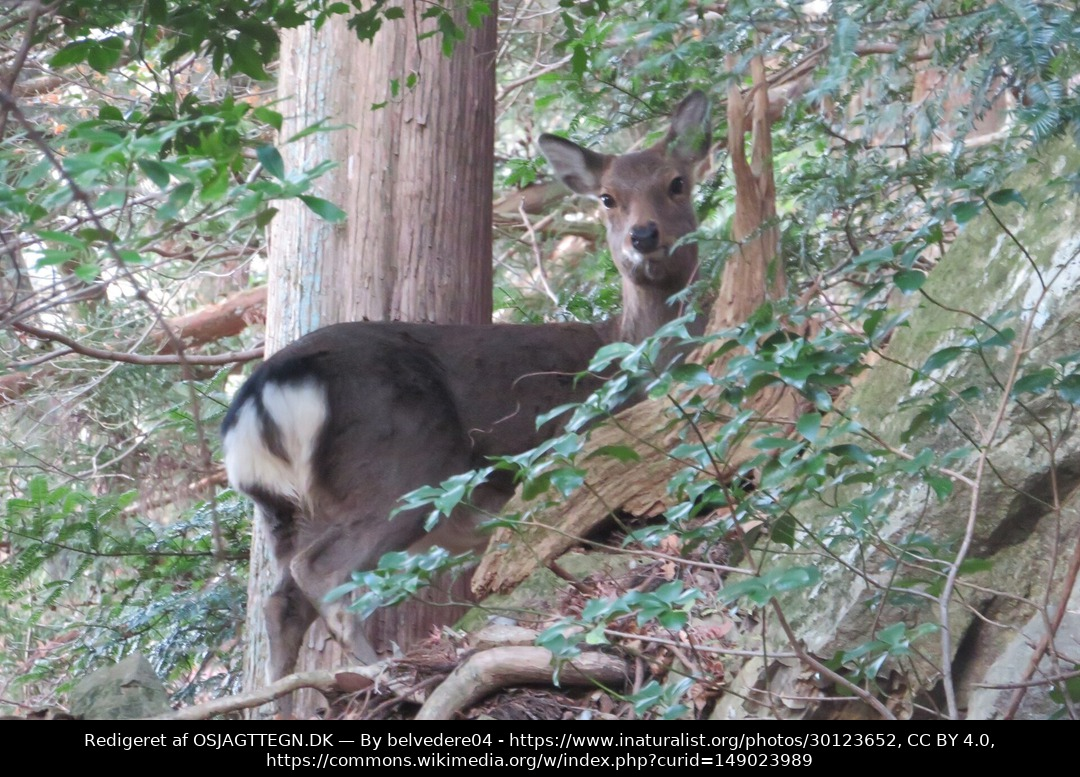
\includegraphics[width=\linewidth, height=7.2cm, keepaspectratio]{Billeder/Dyr/Pattedyr/hovdyr/sikavildt/sikavildt-female-01.jpg}
  \end{columns}
\end{frame}